\documentclass[11pt]{article}


%\documentclass[11 pt]{article}
\usepackage{graphicx}
\usepackage{float}

\usepackage[normalem]{ulem}

\usepackage[utf8]{inputenc}

\usepackage[square,sort,comma,numbers]{natbib}
\bibliographystyle{abbrvnat}
\setcitestyle{authoryear,open={(},close={)}} %Citation-related commands

\usepackage{setspace}

\usepackage{pdflscape}
%\doublespacing
\onehalfspacing
\usepackage[dvipsnames]{xcolor}
\usepackage{lineno}
\linenumbers
\usepackage{multicol}
\usepackage{hyperref}
\hypersetup{
	colorlinks=false,
%	linkcolor=blue,
%	filecolor=magenta,      
%	urlcolor=cyan,
	pdftitle={Overleaf Example},
	pdfpagemode=FullScreen,
}

\addtolength{\oddsidemargin}{-2.5cm}
\addtolength{\evensidemargin}{-1.5cm}

\addtolength{\textwidth}{5.5cm}

\addtolength{\topmargin}{-.875in}
\addtolength{\textheight}{1.75in}

% color can be used to apply background shading to table cells only
%\usepackage[table]{xcolor}

% array package and thick rules for tables
\usepackage{array}

% create "+" rule type for thick vertical lines
\newcolumntype{+}{!{\vrule width 2pt}}

% create \thickcline for thick horizontal lines of variable length
\newlength\savedwidth
\newcommand\thickcline[1]{%
  \noalign{\global\savedwidth\arrayrulewidth\global\arrayrulewidth 2pt}%
  \cline{#1}%
  \noalign{\vskip\arrayrulewidth}%
  \noalign{\global\arrayrulewidth\savedwidth}%
}

% \thickhline command for thick horizontal lines that span the table
\newcommand\thickhline{\noalign{\global\savedwidth\arrayrulewidth\global\arrayrulewidth 2pt}%
\hline
\noalign{\global\arrayrulewidth\savedwidth}}



%\author{Pending}


\begin{document}
%\title{Understanding the emergence of viral variants of concern via Bayesian molecular clock model selection}
\begin{flushright}

%\today
\end{flushright}
\begin{center}
	\begin{LARGE}
	\textbf{The phylodynamic threshold of measurably evolving populations}
	\end{LARGE}

Ariane Weber$^{1,*}$, Julia Kende$^{2}$, Sanni Översti$^{1, \ddagger}$ and Sebastian Duchene$^{3,4,\ddagger, *}$.
\end{center}

$^{1}$ Max Planck Institute of Geoanthropology, Jena, Germany.

$^{2}$ Institut Pasteur, Université Paris Cité, Bioinformatics and Biostatistics Hub, Paris, France.

$^{3}$ ED-ID unit, Dept of Computational Biology, Institut Pasteur, Paris, France.

$^{4}$ Peter Doherty Institute for Infection and Immunity, Dept of Microbiology and Immunology, University of Melbourne, Melbourne, Australia.


*email: weber@gea.mpg.de, sduchene@pasteur.fr
%		\maketitle
\newline

\begin{Large}
	\textbf{Abstract}
\end{Large}
The molecular clock is a fundamental tool for understanding the time and pace of evolution, requiring calibration alongside molecular data. Sampling times are often used for calibration since some organisms accumulate enough mutations over the course of their sampling period. This practice ties two key concepts: measurably evolving populations and the phylodynamic threshold. Current dogma suggests that populations meeting these criteria are suitable for molecular clock calibration via sampling times. However, the definitions and implications of these concepts remain unclear. Using Hepatitis B virus-like simulations and analyses of empirical data, this study shows that determining whether a population is measurably evolving or has reached the phylodynamic threshold depends not just on data, but also on model assumptions and sampling strategies. In Bayesian applications, a lack of temporal signal due to a narrow sampling window results in a prior that is overly informative relative to the data, such that a prior that is potentially misleading typically requires a wider sampling window than one that is reasonable. In our analyses we demonstrate that assessing prior sensitivity is more important than the outcome of tests of temporal signal. Our results offer guidelines to improve molecular clock inferences and highlight limitations in molecular sequence sampling procedures.

\textbf{Keywords:} Measurably evolving population, phylodynamic threshold, molecular clock, Bayesian phylogenetics, microbial evolution.



\section{Introduction}
Molecular sequence data have become nearly ubiquitous for studying the evolution of modern and ancient organisms. A fundamental concept in molecular evolution is the `molecular clock', which posits that substitutions accumulate roughly constantly over time \citep{zuckerkandl1965evolutionary}. An underlying assumption of the classic molecular clock is that selective constraints are negligible for most sites and over time. The development of molecular clock models as statistical processes relaxes this and other assumptions by allowing for rate variation among branches in phylogenetic trees (reviewed by \cite{ho2014molecular, guindon2020rates}).

Molecular clock models necessarily involve two key quantities, the evolutionary timescale and the `evolutionary rate', with the latter representing the combination of mutations and substitutions that accrue over time. However, evolutionary times and rates are unidentifiable (\cite{dos2013unbearable}, as reviewed by \cite{bromham2018bayesian}), and therefore cannot be jointly estimated using genetic sequence data alone. To make inferences about them from genetic sequences, all molecular clock methods require prior assumption about evolutionary times or rates, known as a `molecular clock calibration'. Three main calibrations exist: First, the age of the most recent common ancestor between two samples can be constrained to a given time point or interval (`internal node calibration'). Second, a known estimate of the evolutionary rate can be incorporated (e.g. as a prior in Bayesian frameworks). Third, in cases where molecular sequences are sampled at different points in time (heterochronous sampling), the tips of the phylogeny can be anchored to these time points (`tip calibration'; reviewed by \cite{rieux2016inferences}). The choice of calibration depends on the information available and its reliability \citep{warnock2012exploring, duchene2014impact}. For instance, it would be remiss to ignore evidence about when two lineages shared a common ancestor if the fossil record is compelling. Similarly, multiple sources of calibration information can be provided for the molecular clock.

\subsection{Measurably evolving populations}
Rapidly evolving organisms, notably viruses and some bacteria, have been found to accrue an appreciable number of mutations over the sampling timescale. Influenza viruses, for example, have evolutionary rates of around $6\times10^{-3}$ subs/site/year (substitutions per genomic site per year) \citep{ghafari2022purifying, sanjuan2012molecular}. Assuming a genome size of 13,500 Kb, one would expect to observe one mutation every 4 to 5 days ($\frac{365\ days/year}{13,500\ sites\ \times\ 6\times10^{-3}subs/site/year}\approx4.5\ days/subs$). If genome samples are collected over the course of a few weeks, the sampling times themselves can be used to calibrate the molecular clock and tip calibration is warranted. Data sets for which tip calibration is feasible are considered to have been sampled from a `measurably evolving population' \citep{drummond2003measurably} and to have `temporal signal'. 

Measurably evolving populations are typically characterised either by a sampling period that is long relative to the evolutionary rate, a sufficiently big data set (long molecular sequences or many samples), or both. Traditionally, such characteristics were mainly found in rapidly evolving organisms. Nowadays, advances in sequencing technologies have dramatically expanded the range of organisms from which data sets can be considered to have been sampled from a measurably evolving population. Namely, ancient DNA techniques have effectively expanded the genome sampling window for many organisms \citep{spyrou2019ancient, duchene2020recovery}, and whole genome sequencing has meant that data sets of `slowly' evolving microbes often carry sufficient information for calibrating the molecular clock  \citep{biek2015measurably} even when the sampling period covers only a few decades \citep{menardo2019molecular}.

\subsection{The phylodynamic threshold}
Genomic data sets collected during the early stages of an outbreak, for example, often pose two problems: low genetic diversity and a narrow sampling window. Both can lead to highly uncertain estimates of evolutionary rate and time of origin. The point at which an organism has accumulated sufficient genetic changes since its emergence to allow for informative tip calibration is referred to as the ‘phylodynamic threshold’ \citep{duchene2020temporal}. At a minimum, tip calibration requires that one mutation has occurred over the sampling period for the method to be informative. For a given organism, the minimum sampling period can be calculated as the inverse of the product of genome size and the evolutionary rate (i.e. $\frac{1}{genome\ size\ (sites) \times evol.\ rate (subs/site/year)}=$ years to observe one mutation). We refer to this amount of time as the expected phylodynamic threshold. 

The terms phylodynamic threshold and measurably evolving population are different, albeit related, concepts. A population is measurably evolving if the samples available are sufficiently informative as to allow for tip calibration. In contrast, the phylodynamic threshold is the amount of time over which we would need to draw samples after the emergence for them to behave as from a measurably evolving population. For a recently evolving pathogen the phylodynamic threshold would simply correspond to the time until it can be considered a measurably evolving population, under the condition that the data have been collected constantly over time. In contrast, an organism that emerged further in the past may have accumulated considerable genetic diversity over time, effectively reaching its phylodynamic threshold. However, if samples are drawn from a very short time window they may fail to capture a representative amount of such genetic diversity. 

\subsection{Tests of temporal signal}
Our ability to extract information from a tip calibration framework can be assessed through tests of temporal signal. The importance of performing such tests arises from the observation that a lack of temporal signal is associated with unreliable evolutionary rate estimates \citep{duchene2015performance, rieux2016inferences}, although the presence and direction of a potential bias remain poorly understood. However, it is important to note that a lack of temporal signal does not necessarily preclude estimating evolutionary rates and timescales because alternative sources of calibration, such as prior estimates of evolutionary rates or constraints on internal node ages, can still be used to inform analyses.

In principle, frameworks developed to test for temporal signal do not differentiate between recently emerging organisms (fig. \ref{figure:Fig1}a) and those with narrow sampling windows (fig. \ref{figure:Fig1}d), both of which may lack temporal signal. As most of these tests involve fitting a phylogenetic model to the data, they implicitly assume that the model adequately captures the evolutionary process and thus their performance also highly depends on model fit. Recent research, for example, suggests that the choice of tree prior and molecular clock model significantly impacts the sensitivity and specificity of temporal signal tests \citep{tay2024assessing}. Thus, temporal signal is not solely a property of the data but also depends on model performance.

Various methods exist for assessing temporal signal. The root-to-tip regression \citep{buonagurio1986evolution, gojobori1990molecular, drummond2003inference} fits a regression to the distance from the root to the tips in a phylogenetic tree against sampling time. High $R^2$ values of the regression suggest that phylogenetic distance can be sensibly modelled as a linear function of time and can thus be used as an indication of informative tip-calibration. Date-randomisation tests \citep{ramsden2009hantavirus, duchene2015performance, duchene2018inferring, trovao2015host} compare evolutionary rate estimates using correct sampling times against those from permutations. Bayesian Evaluation of Temporal Signal (BETS; \cite{duchene2020bayesian}) evaluates whether a model with sampling times performs better than a model that assumes isochronous sampling using Bayes factors. Each method comes with a set of limitations and strengths, such that tests of temporal signal should rather be used in combination than being mutually exclusive \citep{rieux2016inferences, duchene2020bayesian}.

\subsection{Concepts of measurably evolving populations, the phylodynamic threshold, and temporal signal in practice}
In fig. \ref{figure:Fig1}, we present four simple example cases to illustrate the relationships among the concepts of measurably evolving populations, the phylodynamic threshold, and temporal signal. The first example depicts an organism that has emerged recently and therefore has not yet reached its phylodynamic threshold (with a phylogenetic time tree shown in panel (a)). Due to its recent origin, there has not been enough time for the accumulation of a sufficient number of substitutions (represented in the phylogram in panel (b)), such that it is not possible to establish a statistical relationship between molecular evolution (i.e., substitutions) and time (as shown in panel (c)). A real-world example of such a case comes from the early phase of the SARS-CoV-2 outbreak: initial efforts to estimate the evolutionary rate and time of origin had substantial uncertainty due to a narrow sampling window and low genetic diversity \citep{boni2020evolutionary}. In \cite{duchene2020temporal}, Bayesian phylodynamic analyses were conducted on genome data as the outbreak unfolded. The number of available genomes and the width of the sampling window increased over time and ranged from 22 genomes sampled over 31 days to 122 genomes sampled over 63 days. Although early estimates of the evolutionary rate and time of origin were highly uncertain, they quickly converged to stable values as more data became available \citep{ghafari2022purifying}. 
   
The second example in fig. \ref{figure:Fig1} illustrates a case in which an organism has evolved over a long period, but the available sequence data have been collected within a very narrow timeframe, insufficient to treat the dataset as a measurably evolving population (time tree in panel (d) and phylogram in panel (e)). This results in no temporal signal, as demonstrated by the lack of correlation in the root-to-tip regression in panel (f). The causative agent of tuberculosis, the bacterium \textit{Mycobacterium tuberculosis}, was commonly considered to evolve too slowly for calibrating the molecular clock using samples collected over a few years \cite{duchene2016genome}. Later studies have shown, however, that for \textit{M. tuberculosis} a genome sampling window of a few decades might be sufficient for reliable clock calibration \citep{menardo2019molecular, kuhnert2018tuberculosis, merker2022transcontinental}. 
 
The third example in fig. \ref{figure:Fig1} describes a data set that may involve a wide sampling window of time and for which samples have been drawn from a population that has attained its phylodynamic threshold, but with substantial rate variation among lineages – i.e. overdispersed molecular clock -,  resulting in a lack of temporal signal (panels (g) – (i)). This pattern appears to be the case in \textit{Yersinia pestis}, the bacterium that causes the plague, for which some localised outbreaks display obvious temporal signal, but its long-term evolution has pervasive evolutionary rate variation \citep{eaton2023plagued, andrades2022stone}. 

In the final example in fig. \ref{figure:Fig1}, a hypothetical organism has attained its phylodynamic threshold, has been sampled for sufficiently long time, and evolutionary rate variation among lineages is low. These conditions together produce a clear relationship between molecular evolution and time, thus providing unequivocal temporal signal (panels (j) – (l)). The long term evolution of \textit{Vibrio cholerae}, the causative agent of cholera, and H3N2 influenza virus are exemplar microbes whose molecular evolution has been fairly constant across long periods of time \citep{devault2014second, rambaut2016exploring}.

In summary, the concepts of measurably evolving population, phylodynamic threshold and temporal signal describe the information that can be drawn from a sampled population about its evolutionary timescale. Because populations that are not measurably evolving have been observed to yield biased estimates, they remain important to consider \citep{gharbi2024clock}. In Bayesian inference, such biases can be the result of complex interactions between prior distributions or model settings that do not align with the true data generating model, as these drive the inference in the absence of informative data. Traditionally, potential biases due to prior interactions \citep{tay2024assessing} or model misspecification \citep{moller2018impact} have been found through simulations studies, while data analyses often involve little validations of the results \citep{mendes2025validate}. Here, we illustrate through a range of examples the degree to which differing levels of temporal signal in a data set can interact with prior settings and model assumptions, both on simulated and empirical data. 
\section{Results}
We sought to pinpoint the impact of sampling strategies on molecular clock estimates. We focused our attention on two major problems for emerging microbes and studies involving ancient DNA. First, we conducted simulations varying the sampling window of a population that had attained its phylodynamic threshold. In the second simulation scenario, we subsampled a population over time to vary the number of ancient samples, leading to a temporal sampling bias. Finally, we illustrate these results in an empirical data set of Hepatitis B virus (HBV) that includes a large number of ancient samples \citep{kocher2021ten}. This virus has been the subject of intense research due to its close association with human populations and complex evolutionary dynamics \citep{paraskevis2013dating, ross2018paradox, kahila2012tracing}.

\subsection{Sampling windows relative to the phylodynamic threshold}
We simulated sequence data that resembled the evolution of HBV, a double-stranded DNA (dsDNA) virus that has evolved in humans at least for around ten thousand years \citep{kocher2021ten}. Our synthetic data had a genome length of 3,200 nucleotides and an evolutionary rate of $1.5\times10^{-5}$ subs/site/year \citep{kocher2021ten, muhlemann2018ancient} with a moderate amount of rate variation among lineages (see Materials and methods). Under these conditions we expect to observe one mutation every 20 years ($\frac{1}{3,200\ sites \times\ 1.5\times10^{-5}subs/site/year}\approx20\ years/subs$). This number is important for the design of our simulation experiments: 20 years is the expected phylodynamic threshold, as introduced above, and typically serves as a good reference point from when on to expect temporal signal. We analysed the data under a Bayesian phylogenetic framework and considered whether the posterior contained the true value used to generate the data, known as coverage, and the width of the posterior, known as precision (a precise estimate has a narrow posterior distribution).

We conceived a simulation process under which the evolutionary timescale had an expectation of ten thousand years and with a sampling window of 0, 10, 20, 200 , or 2,000 years. A sampling window spanning 0 years results in ultrametric trees with the sampling times providing no calibration information. In contrast, a sampling window of 10 years is half of the expected phylodynamic threshold and is likely to have weak temporal signal (see fig. \ref{figure:Fig1}(d)-(f)). Sampling windows of 20 years (the expected phylodynamic threshold) or wider are more likely to behave as measurably evolving populations with increasingly strong temporal signal (see fig. \ref{figure:Fig1}(j)-(l)). All of our simulations were analysed under Bayesian phylogenetic framework, as implemented in the BEAST 2 platform \citep{bouckaert2019beast}.

\begin{landscape}
	\begin{figure}[H]
		\begin{center}
			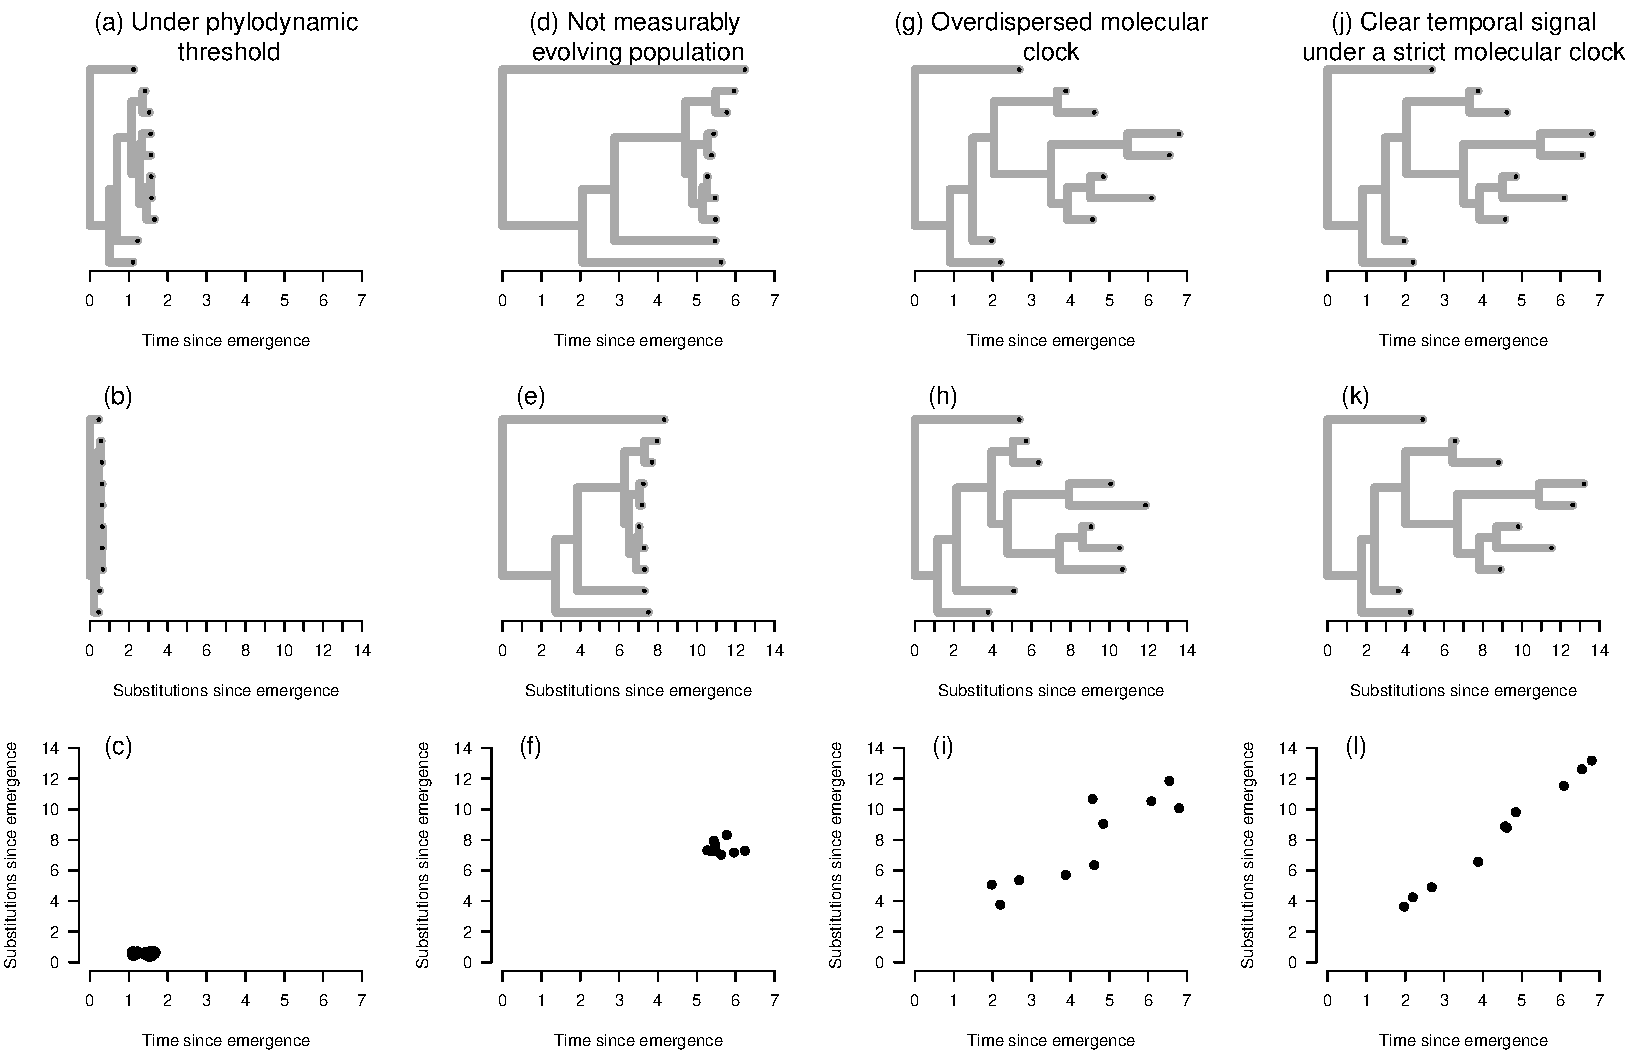
\includegraphics[scale=0.55, angle=0]{examples_temp_signal_thresholds_meps.pdf}
			\caption{Examples of situations where temporal signal may or may not be detected. An organism that has not attained its phylodynamic threshold has a recent time of emergence (with a phylogenetic time tree shown in (a)) because it has not had sufficient time to accrue an appreciable number of substitutions (phylogenetic tree with branch lengths in subs/site, i.e. a `phylogram', shown in (b)), such that it is not possible to establish a statistical relationship between molecular evolution (substitutions) and time (shown in (c)). Sequence data from an organism that has evolved for a substantial amount of time may have been sampled over a very narrow window of time that is not sufficient to treat it as a measurably evolving population (time tree in (d) and phylogram in (e)), which results in no temporal signal (root-to-tip regression in (f)). A data set may involve a wide sampling window of time and from a population that has attained its phylodynamic threshold, but an overdispersed molecular clock (substantial rate variation among lineages; panels (g) - (i)) may result in a lack of temporal signal. In (j) through (l) we show the situation where an organism has attained its phylodynamic threshold, it has been sampled for sufficiently long, and where evolutionary rate variation among lineages is negligible, as to produce a clear relationship between molecular evolution and time, and thus unequivocal temporal signal.}
			\label{figure:Fig1}
		\end{center}
		%		\centering
	\end{figure}
\end{landscape}

All our simulations produced posterior estimates that included the correct value used to generate the data (i.e. 100\% coverage; fig. \ref{figure:Fig2}). Increasingly wide sampling windows improved the precision of the estimates, while still including the correct value. This result is unsurprising, given our configuration of the prior. Here, the tree prior is a constant-size coalescent for which the prior on the population size (known as $\theta$) is an exponential distribution with mean of 5,000, which matches the value used to generate the data. Similarly, the evolutionary rate had a prior in the form of a $\Gamma$ distribution with $shape=1.5$ and $rate=10^{5}$, whose mean is $shape\times rate=1.5\times10^{-5}$ and thus also matches the `true' value. Although these priors are centred on the correct values, they are vague, and it is important to note that in all cases, the posterior distributions of the evolutionary rate and tree height were narrower than their priors, meaning that even in the absence of sampling times the sequence data themselves provide some information about these two parameters.

We reanalysed these data with deliberately `misleading' priors on the population size and the evolutionary rate. The prior on the population size was an exponential distribution with mean of 50,000, whereas the prior on the evolutionary rate was $\Gamma(shape=1.5, rate=10^{6})$ (mean=$1.5\times10^{-6}$). Under this configuration the mean prior mass corresponds to trees that are one order of magnitude older than the truth and evolutionary rates that are an order of magnitude slower. The objective of this experiment is to determine whether the sampling window is sufficiently informative to overcome such misleading prior information.

The posterior distribution was largely contained within the prior, resulting in low coverage for the evolutionary rate for sampling windows of 0, 10, and 20 years (0\% coverage; fig. \ref{figure:Fig3}). A sampling window of 200 years was necessary to obtain 92\% coverage, while a sampling window of 2,000 years had 100\% coverage and even higher precision (fig. \ref{figure:Fig3}). These results demonstrate that a misleading prior that places a very low probability on the true value, requires a sampling window that is potentially much wider than the expected phylodynamic threshold. 

Contrary to the expectation that low temporal signal necessarily results in an underestimation of the evolutionary rate and an overestimation of the tree height \citep{duchene2015performance}, we find that a lack of temporal signal due to narrow sampling windows may simply lend more influence to the prior. To confirm this point we conducted and additional set of simulations where the mean evolutionary rate prior was $\Gamma(shape=1.5, rate=10^{4})$ (mean=$1.5\times 10^{-4}$, and 95\% range from $1.08 \times 10^{-5}$ to $4.7 \times 10^{-4}$), and thus should lead to an overestimation of this parameter. As expected, we also found that increasing the width of the sampling window resulted in a prior that was less influential on the posterior and with the latter converging to the value used to generate the data (see Supplementary material). Compared to the previous setting with incorrectly lower prior, a narrower sampling window already resulted in good coverage. This is unsurprising, as higher rate values are less likely when only few mutations are observed in a relatively long sampling window, while lower rate values cannot be excluded.

\begin{landscape}
	\begin{figure}[H]
		\begin{center}
		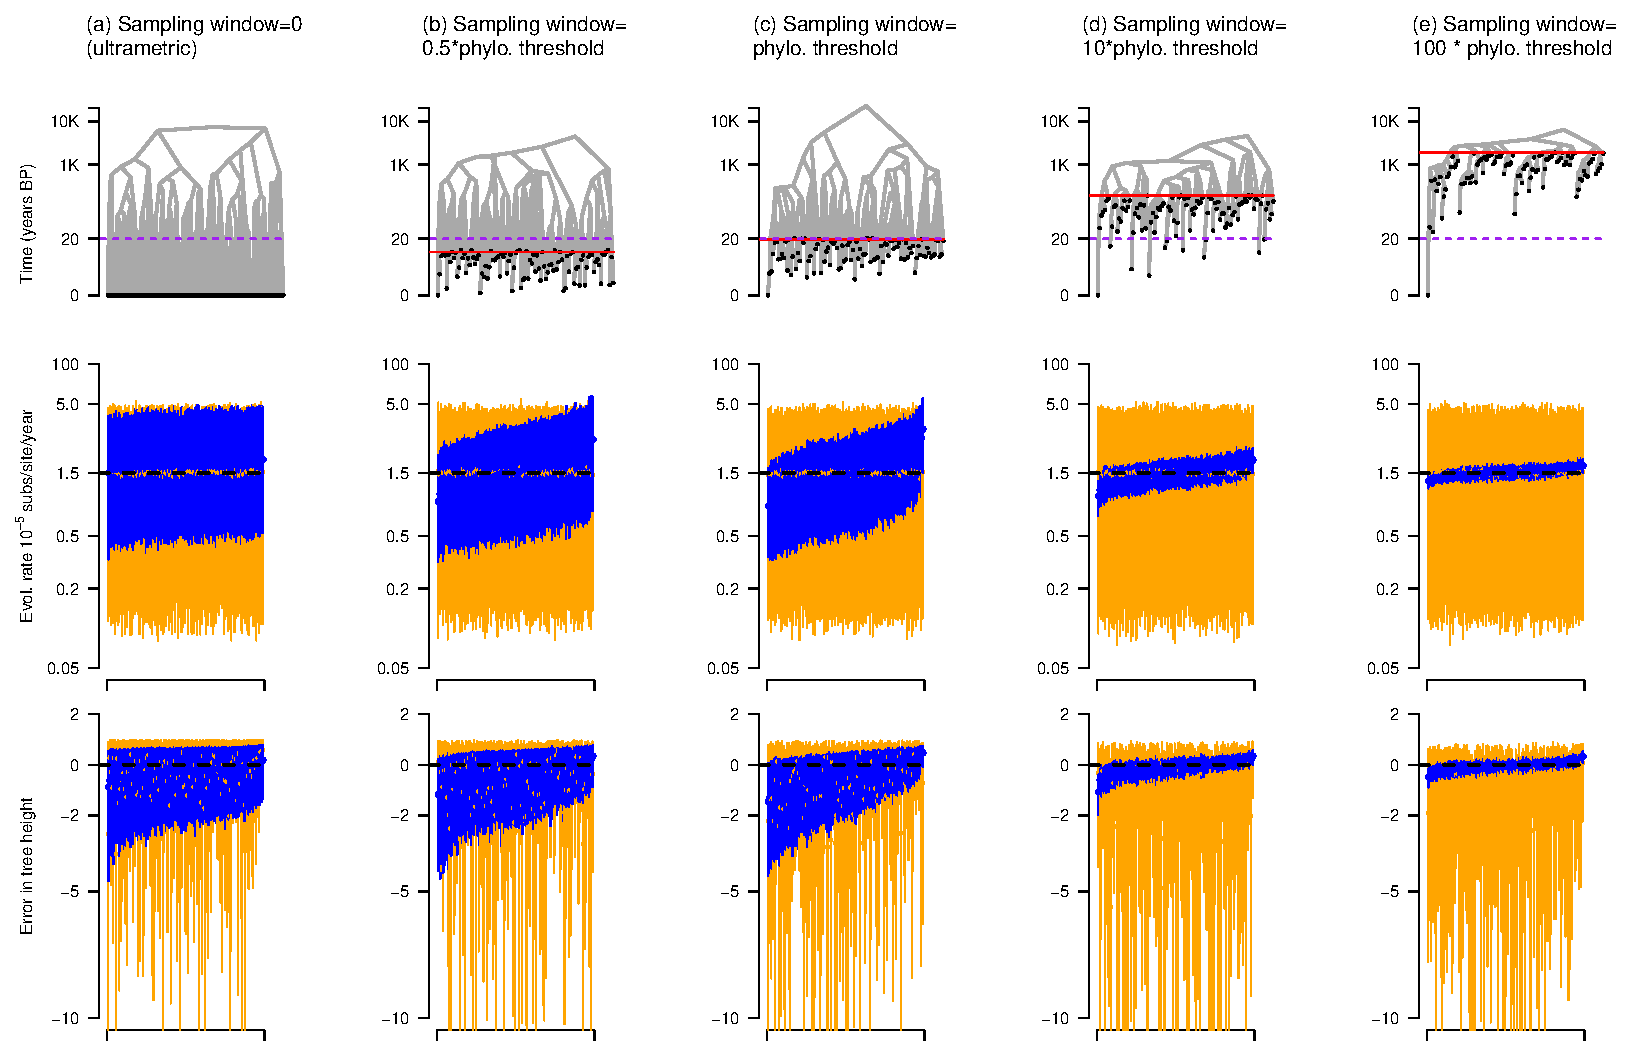
\includegraphics[scale=0.7, angle=0]{summary_all_estimates_correct_prior.pdf}
			\caption{Simulations of varying sampling window widths. Each column corresponds to a simulation setting: (a) is for ultrametric trees where all samples are collected at the same point in time, (b) is for the situation where the sampling window is 10 years (half the expected phylodynamic threshold), (c) is where the sampling window is exactly the expected phylodynamic threshold of 20 years. Scenarios (d) and (e) denote sampling windows that are 10 and 100 times the expected phylodynamic threshold. The first row is an example of a simulated phylogenetic tree with branch lengths scaled in units of time. The black circles represent genomic samples. The purple dashed line is the expected phylodynamic threshold and the solid red line is for the oldest sample, such that it represents the sampling window. Note that time here is shown in log$_{10}$ scale. The second row is the estimated evolutionary rate over 100 simulations. The dashed black line is the value used to generate the data (i.e. the ground truth), the dark blue bars are the posterior, and those in orange are the prior. For the prior and the posterior we use solid circles to show the mean estimate and the width of the error bars denotes the 95\% quantile range. The third row is the estimate of the error in tree height (the age of the tree). The error in tree height is calculated as $\frac{true-estimated}{true}$.}
			\label{figure:Fig2}
		\end{center}
		%		\centering
	\end{figure}
\end{landscape}

\begin{landscape}
	\begin{figure}[H]
		\begin{center}
			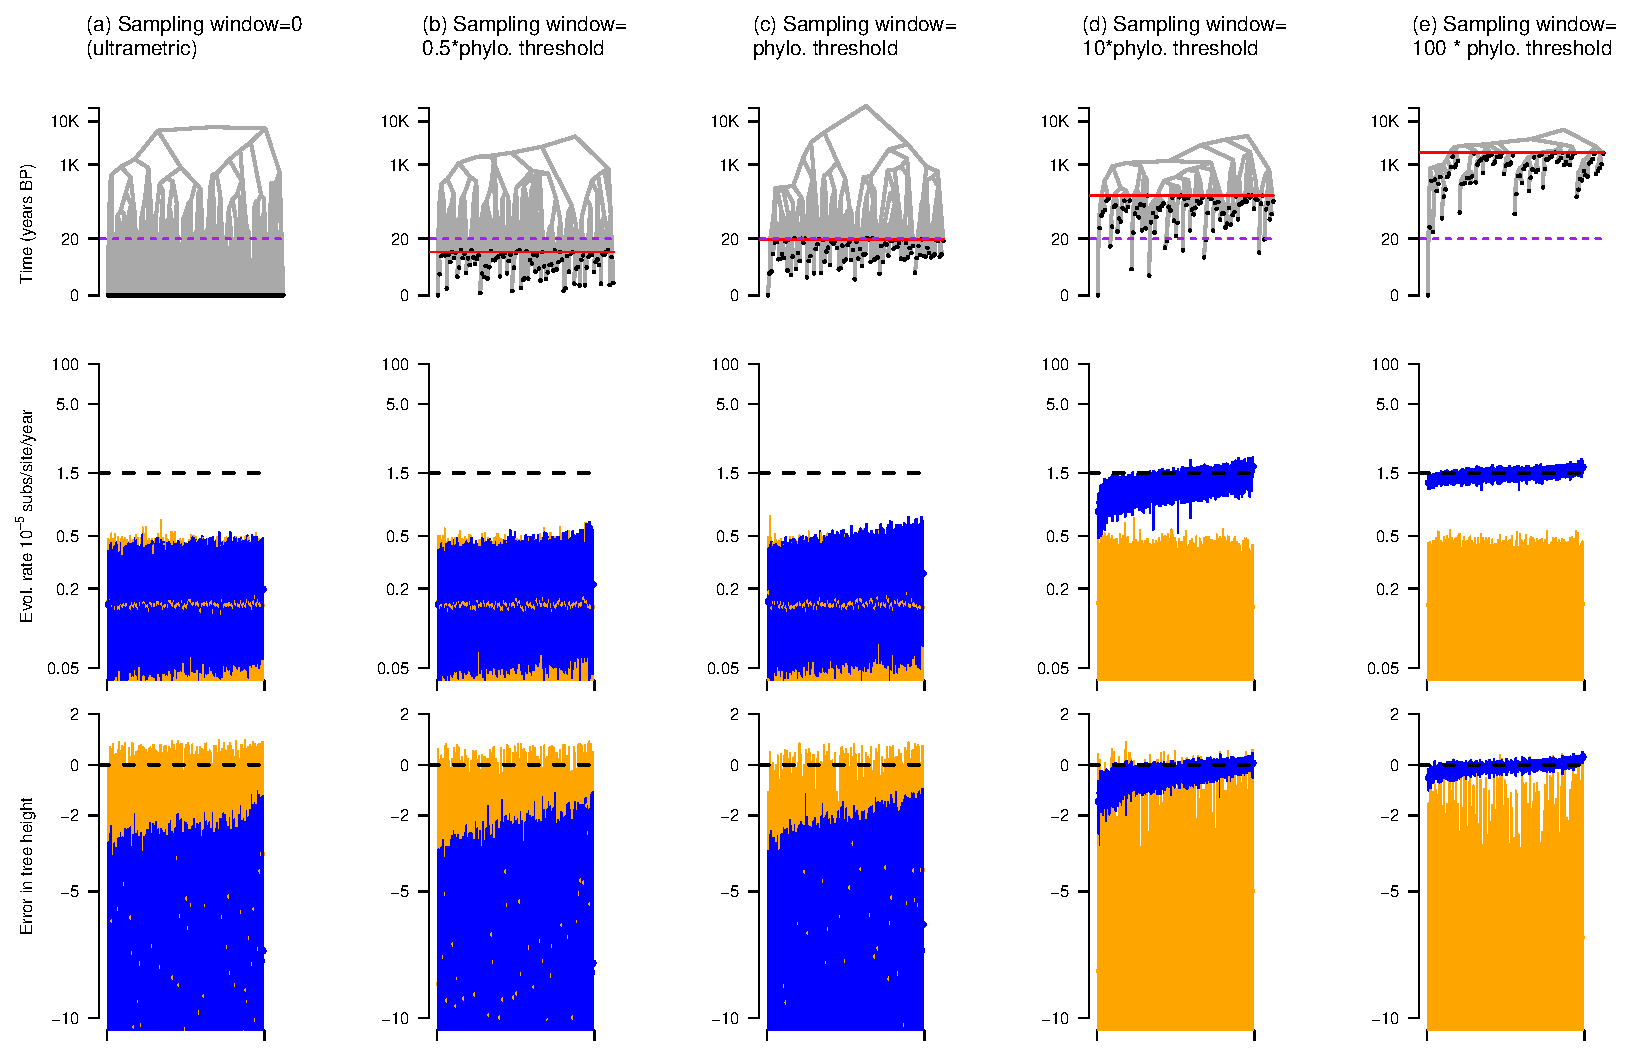
\includegraphics[scale=0.7, angle=0]{summary_all_estimates_misleading_prior.pdf}
			\caption{Simulations of varying sampling window widths. The colours, labels and legends match those from fig \ref{figure:Fig2}. However, in these analyses we deliberate use misleading priors on two key parameters, with a exponential distribution with mean 5,000 for the coalescent population size (true value=5,000), and a $\Gamma(shape=1.5, rate=10^{6})$ with mean=$1.5\times10^{-6}$ (true value=$1.5\times10^{-5}$).}
			\label{figure:Fig3}
		\end{center}
		%		\centering
	\end{figure}
\end{landscape}


\subsection{Temporal sampling bias}
We investigated the impact of temporal sampling bias on the precision and accuracy on molecular clock estimates. For this purpose we simulated data with the same genomic characteristics as HBV and where genome sampling was conducted over five periods of time uniformly distributed between the present and the root of the trees (fig. \ref{figure:Fig4}(a)). The fully sampled trees contained 500 genome samples, with 100 for each of the five sampling times. Such stratified sampling is expected in ancient DNA studies, for example when a set of samples are drawn from archaeological sites (e.g. \cite{spyrou2019phylogeography}). We sampled the complete data sets by randomly selecting 20 samples from each strata, which we refer to as `time-uniform' sampling, and by sampling with a probability that is inversely proportional to the age of the strata, referred to as `time-biased'. The time-uniform and time-biased sampling strategies both contain 100 samples (1/5$^{th}$ of the complete data), but the time-biased only includes a small number of ancient samples.

The coverage of the evolutionary rate estimate was comparable across simulation treatments, at 88\% for the complete data set, 83\% for the time-uniform, and 89\% for the time-biased (fig. \ref{figure:Fig4}(b)). The somewhat higher coverage for the estimates from the time-biased analyses is likely because this sampling treatment has the lowest precision in the posterior, rather than an improvement in both accuracy and precision.

We also calculated a measure of bias for both sampling strategies by counting the number of simulations for which the posterior mean with either sampling strategy was higher than that with the complete data. We found that 50\% of the estimates under time-uniform sampling had higher means than the complete data, while the same was true for 45\% of those with time-biased sampling (fig. \ref{figure:Fig5}(a)). Although these numbers do not indicate substantial bias, such as a systematic over- or underestimation, we do note that time-biased sampling tends to produce lower mean evolutionary rate estimates than those obtained from the complete data or time-uniform sampling.

The most striking result of the temporal sampling strategies was in the precision of the posterior. Both sampling treatments resulted in posterior distributions that were wider than with the complete data, which is to be expected because they are effectively smaller data sets with less information. However, the time-biased sampling data sets almost invariably have posterior distributions that were less precise than those from the time-uniform sampling (Fig. \ref{figure:Fig5}(b)), implying that the distribution of samples, and not just the number, is important for estimation precision.

%\begin{landscape}define preempt
\begin{figure}[H]
	\begin{center}
		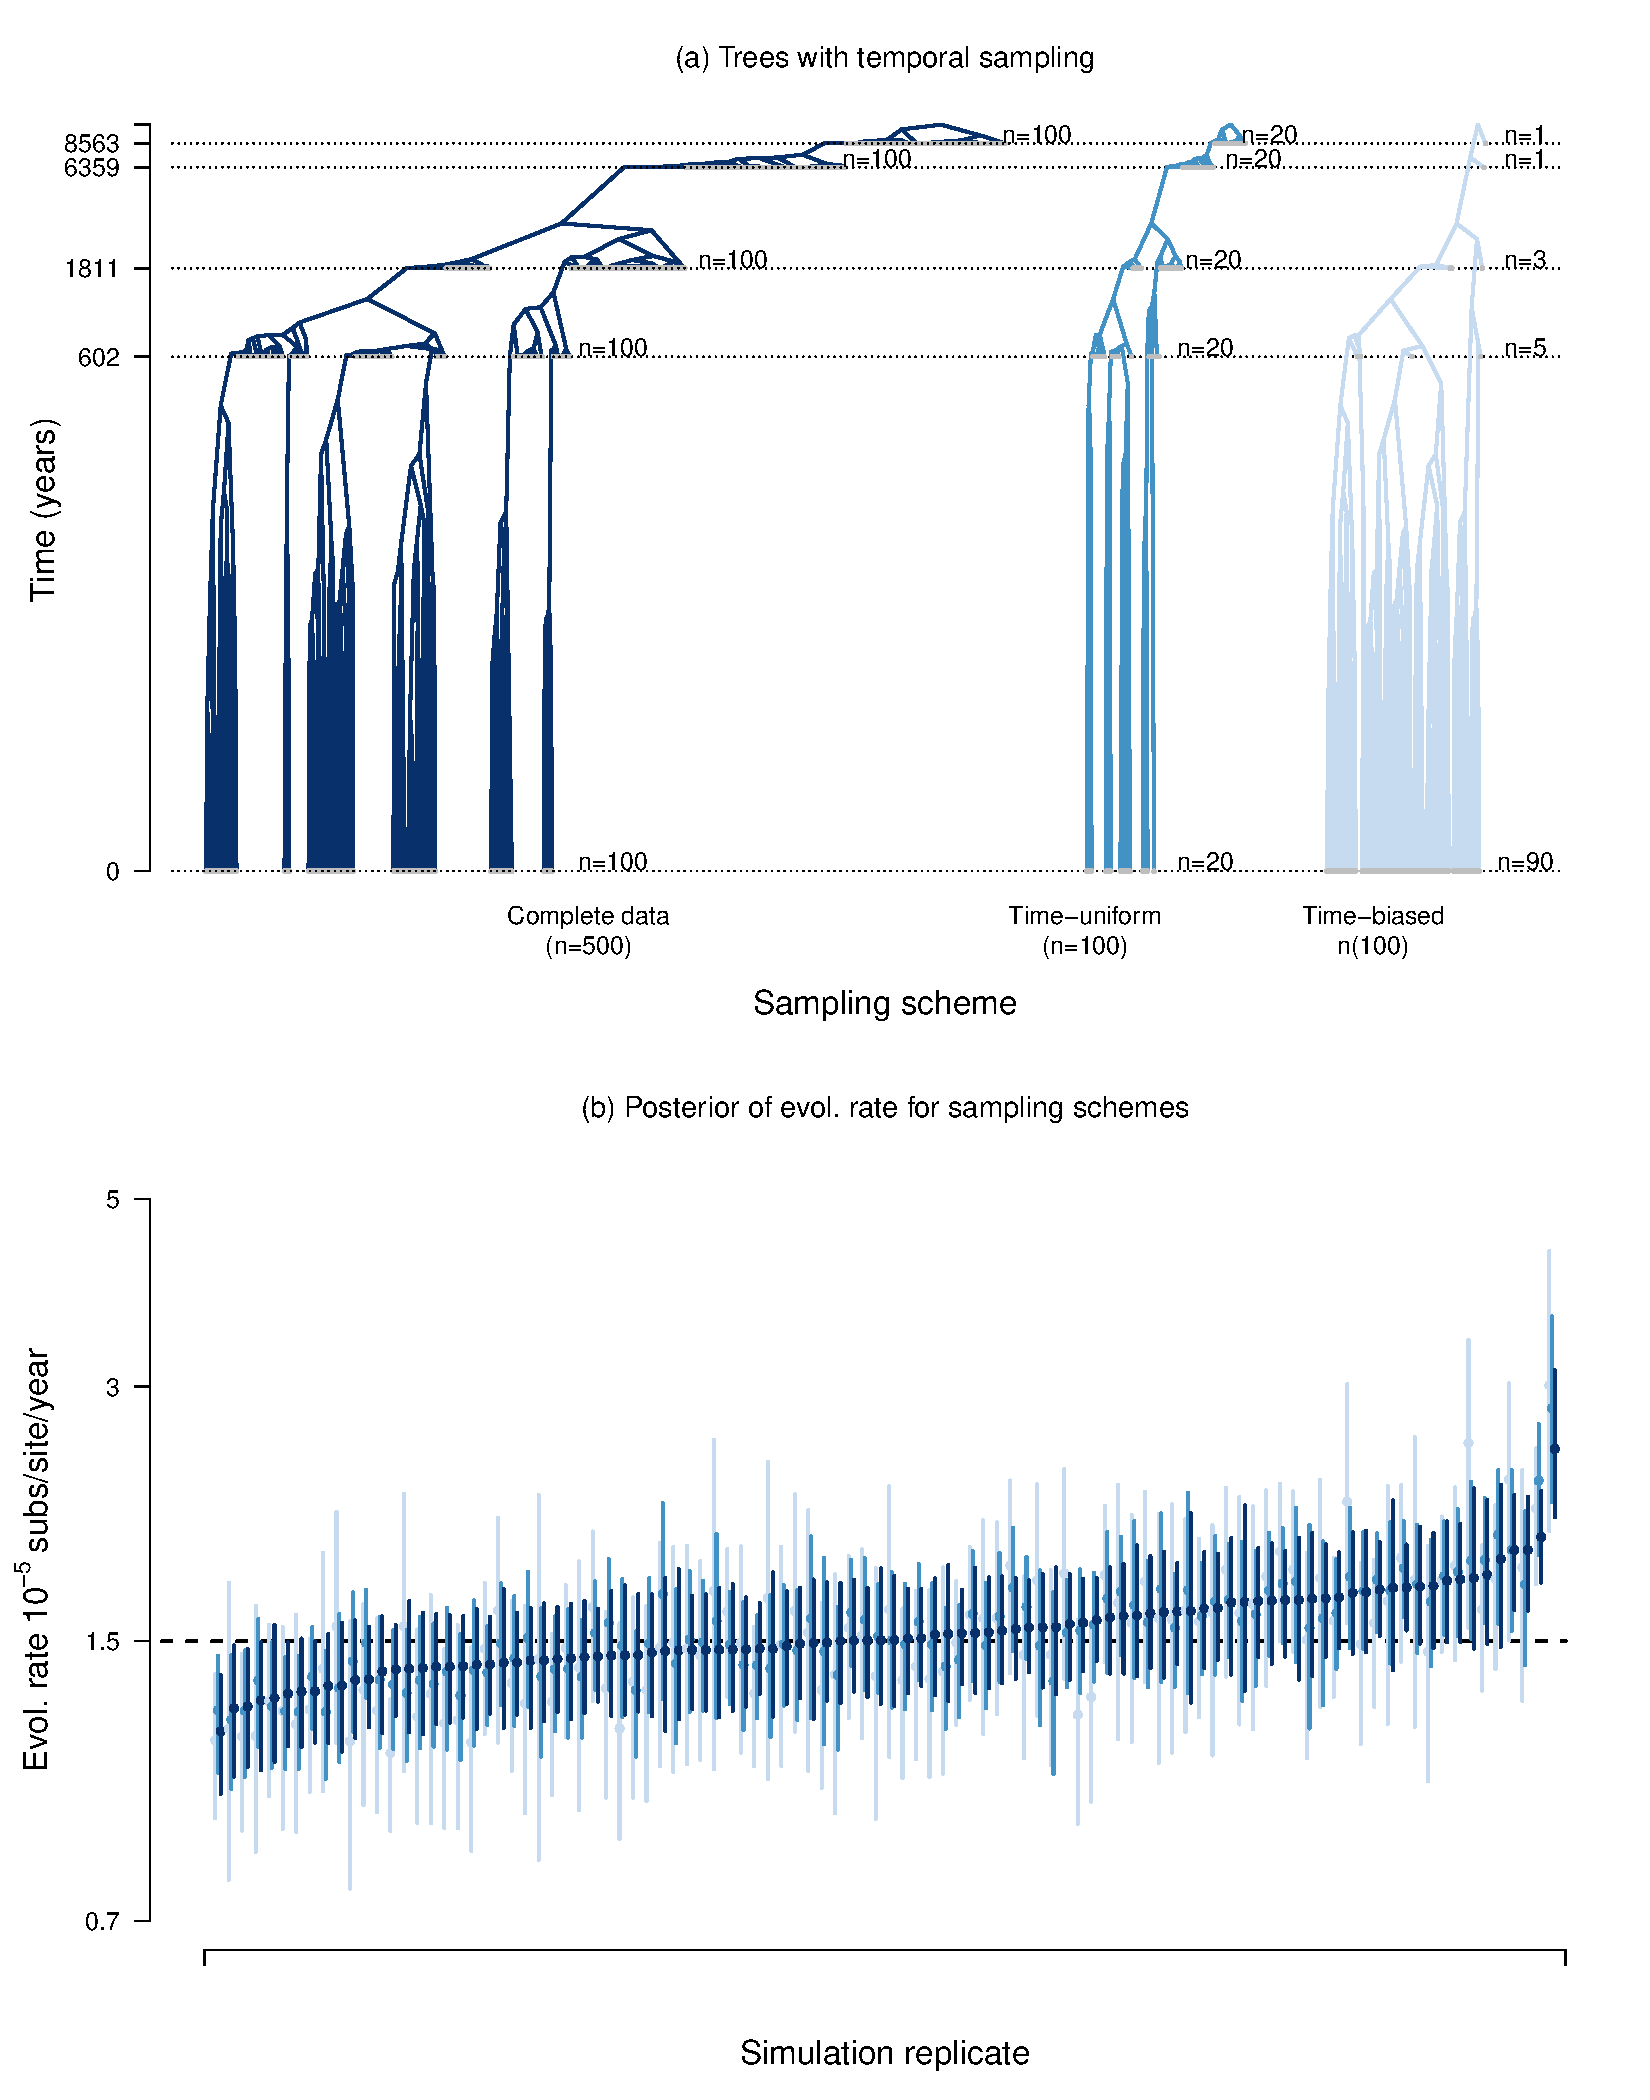
\includegraphics[scale=0.5, angle=0]{sampling_bias_summary_trees_rates.pdf}
		\caption{Analyses under sampling treatments over time. In (a) we show an example of the trees for a simulation replicate, with branch lengths and time in log$_{10}$ scale. The complete data set consists of 500 genome samples, collected in five points in time, with an equal number of samples per time point (n=100). The first sampling strategy is unbiased, where 20 samples are drawn from each time point, and is known here as `time-uniform'. The `time-biased' regime is where sampling intensity decreases over time. Note that the total number of samples in the time-uniform and time-biased treatments is identical. In (b) we show the posterior estimates of the evolutionary rate for each treatment. Each simulation replicate is represented by three error bars: dark blue for the complete data, and lighter shades of blue for the estimates from the time-uniform and time-biased sampling treatments. The width of the error bars denotes the 95\% quantile range and the dots are the mean value. The dashed line shows the true value used to generate the data.}
		\label{figure:Fig4}
	\end{center}
		%		\centering
\end{figure}
%\end{landscape}


\begin{figure}[H]
	\begin{center}
		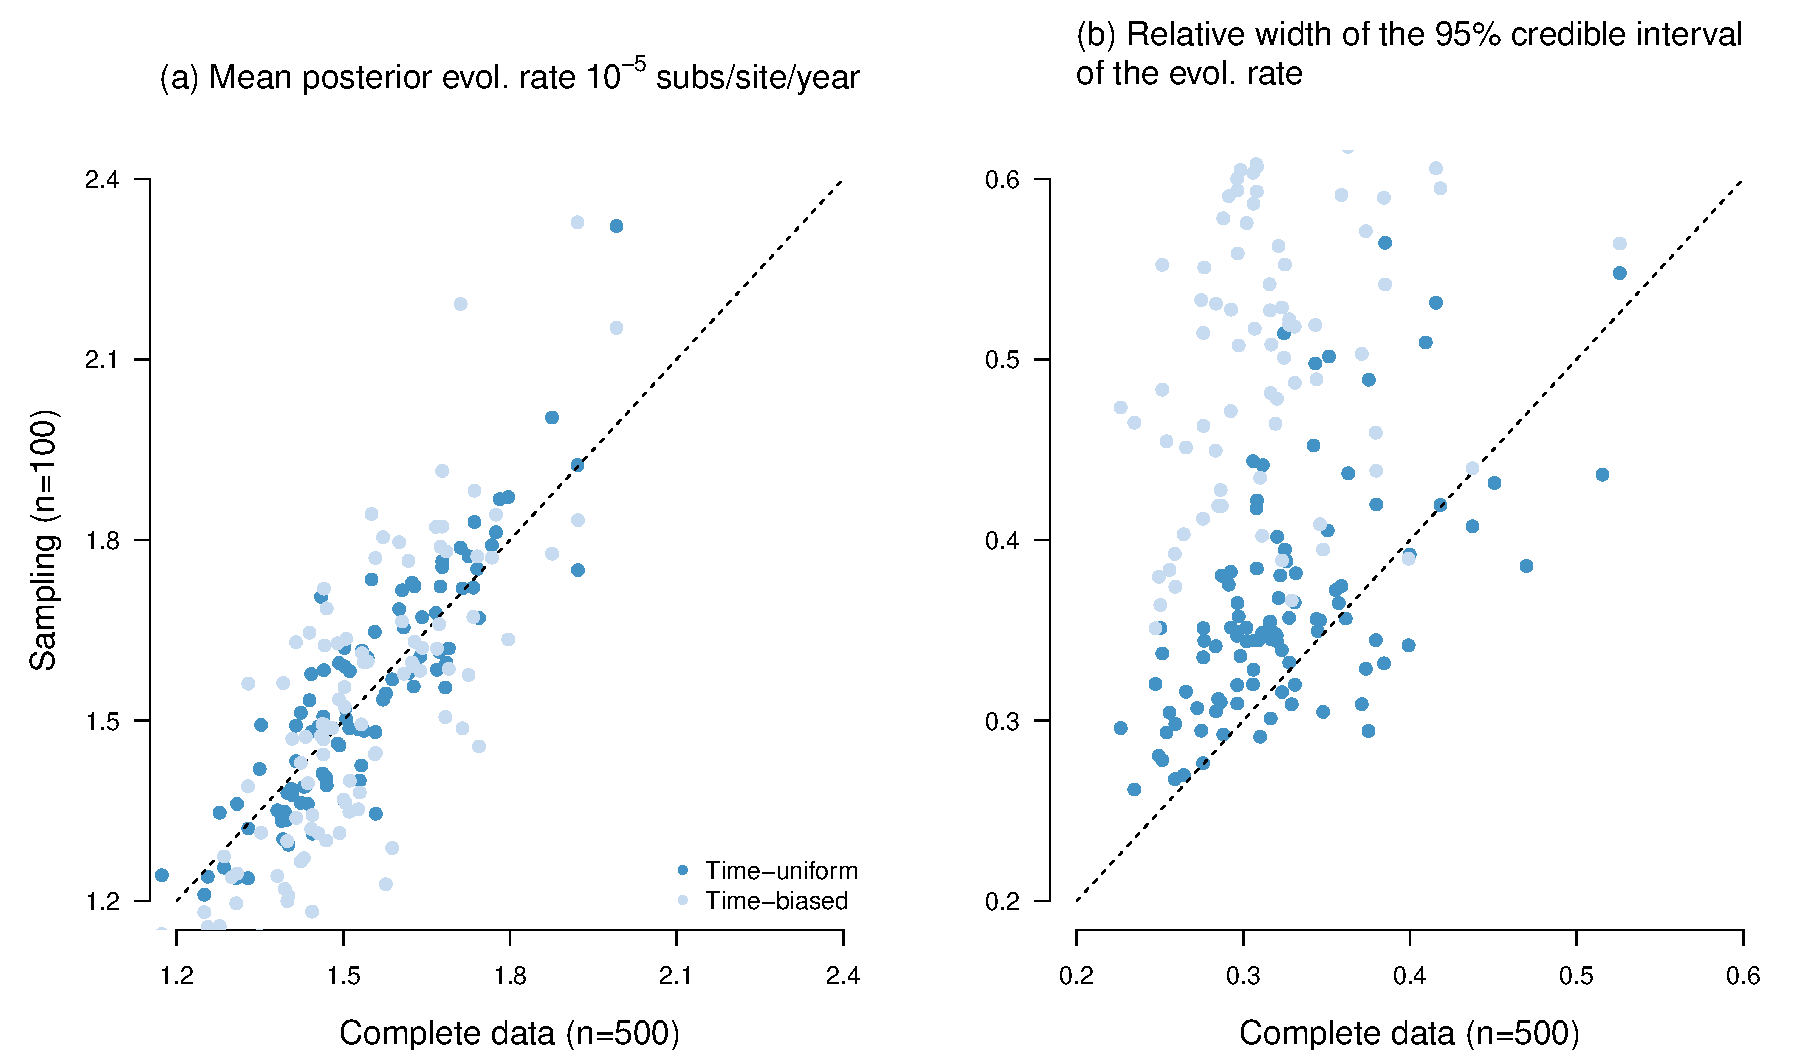
\includegraphics[scale=0.5, angle=0]{sampling_bias_summary_rates.pdf}
		\caption{Comparison of posterior evolutionary rate estimates between complete data (x-axis) and two sampling treatments (y-axis): time-uniform (dark blue) and time-biased (light blue). Each dot is a simulation replicate. In (a) we show the mean posterior evolutionary rate estimate. Points that fall along the y=x line (dashed line) represent identical mean posterior for the sampling treatment and the complete data, while those above or below represent higher or lower estimates, respectively, relative to the complete data. In (b) we show the width of the credible interval (a measure of precision or uncertainty), calculated as the upper minus the lower 95\% credible interval range divided by the mean value. Values that fall along the y=x line denote those for which the complete data and either sampling strategies are equally precise, while those above and below the y=x line are more or less precise, respectively.}
		\label{figure:Fig5}
	\end{center}
	%		\centering
\end{figure}

\subsection{Empirical analyses of Hepatitis B virus (HBV) ancient and modern genomes}
To explore the impact of the width of the sampling window and the temporal sampling bias on the estimates of evolutionary rates and times, we performed analyses of a HBV data set that includes modern and ancient genomes, from \cite{kocher2021ten}. The complete data set consisted of 232 genomes of length 3,344 nucleotides and with a sampling window of 10,535 years. HBV is an ancient pathogen that has likely codiverged with human populations for thousands of years \citep{locarnini2021origins, zehender2014enigmatic, paraskevis2013dating, muhlemann2018ancient}, and thus its phylodynamic threshold has been reached while it has not been empirically established if it can be considered to be a measurably evolving population, as is the case for recent outbreaks, like SARS-CoV-2 \citep{duchene2020temporal}. 

For our first set of analyses we varied the width of the sampling window. We drew 100 genomes with different sampling window widths: 0 (only modern samples), up to 500, 1,000, or 5,000 years before present. Increasing the sampling window resulted in estimates of the evolutionary rate that were more precise and closer to the estimate from the complete data set (fig. \ref{figure:Fig6}). Here we find that the evolutionary rate is estimated to be higher for shorter sampling windows, with correspondingly older estimates for the tree height (see Supplementary material). This pattern can be due to one or a combination of other factors influencing the inference, for example the vagaries of evolutionary rate variation in this virus, particularly time-dependency \citep{vrancken2017accurate}. Similarly, population structure that is unaccounted for has been shown to produce an overestimation of the evolutionary rate, because under the tree prior samples that are genetically linked are expected to have been sampled at the same point in time \citep{moller2018impact}.

\begin{figure}[H]
    \begin{center}
        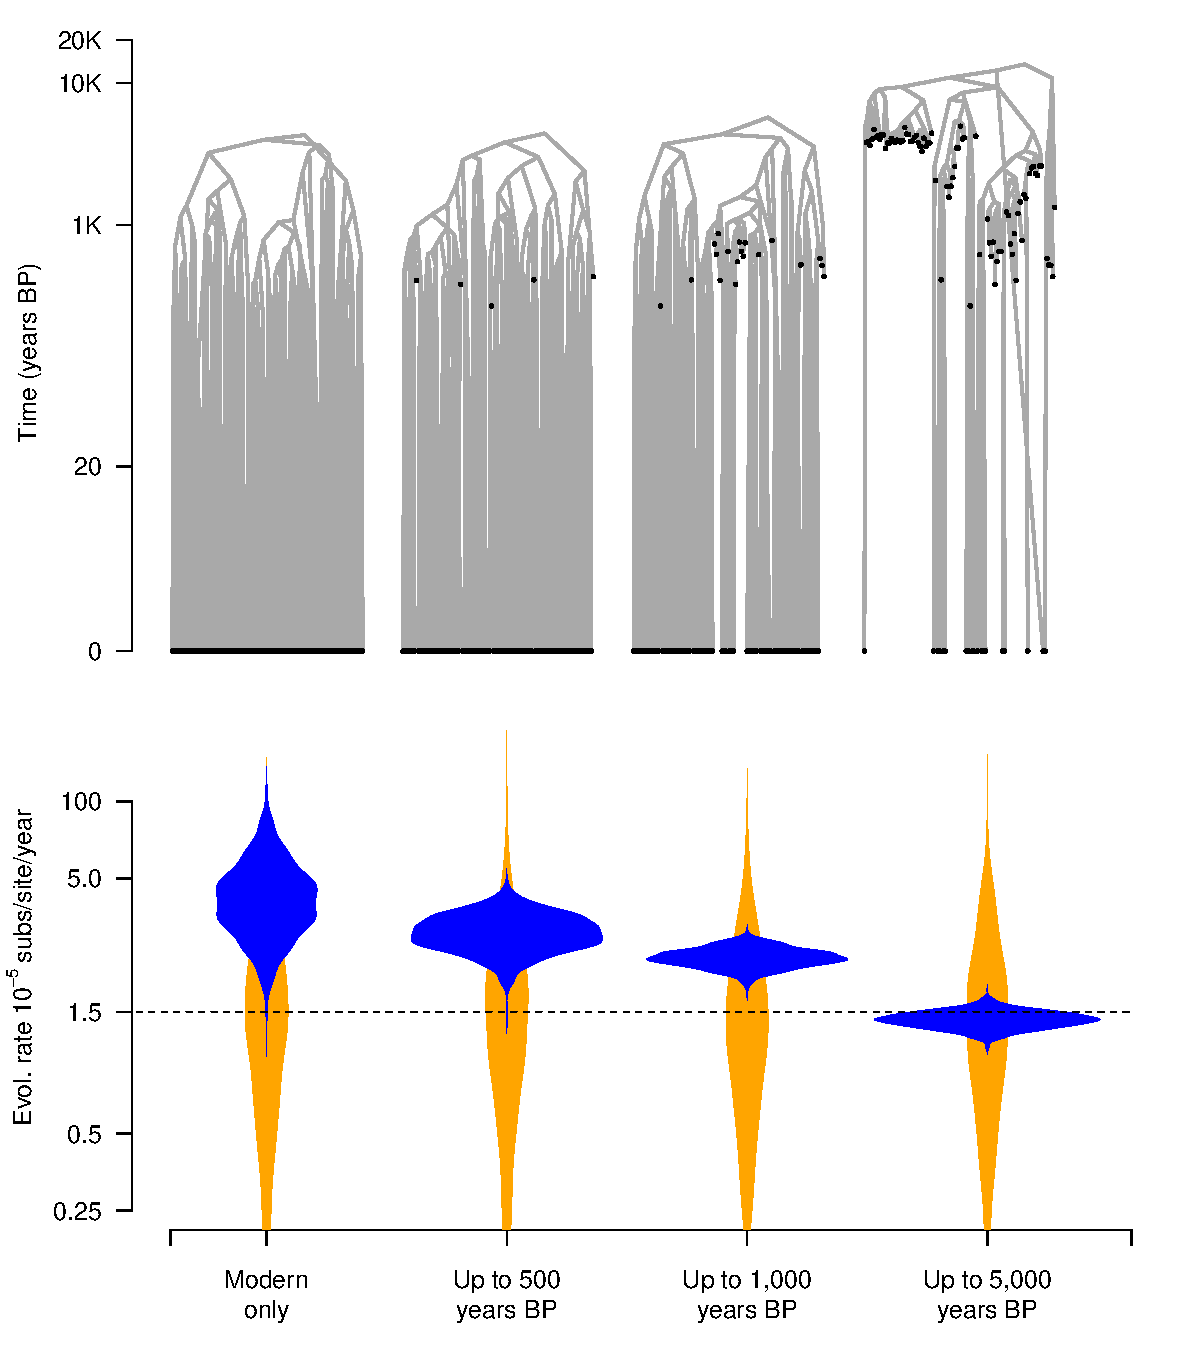
\includegraphics[scale=0.7, angle=0]{empirical_results_depth.pdf}
        \caption{Results from empirical analyses of Hepatitis B virus (HBV) ancient DNA data. The phylogenetic trees correspond to highest clade credibility trees from three analyses where the data were subsampled to increase the width of the sampling window progressively. First, we only consider modern samples, then those up to 500, 1,000, and 5,000 years before present. In all cases the data sets consist of 100 genome samples. The violin plots show the posterior distribution of the evolutionary rate in blue and its corresponding prior in orange. The dashed line shows the mean evolutionary rate estimate from the complete data set.}
        \label{figure:Fig6}
    \end{center}
    %		\centering
\end{figure}

For our second set of empirical analyses, we subsampled the data to produce a range of temporally biased sampling scenarios. We varied the proportion of modern samples, from 95\% to 10\%. Here the sampling window is constant because we always retain the most ancient samples. Each data set consisted of 100 genomes, such that they only differ in the distribution of modern and ancient samples (fig. \ref{figure:Fig7}). 

The impact of temporal sampling bias was less clear than in our simulations above (figs \ref{figure:Fig4} and \ref{figure:Fig5}). The data set with 95\% modern genomes had the highest uncertainty in the evolutionary rate estimate, but uncertainty did not decrease monotonically with the proportion of modern genomes. Moreover, the posterior estimate of the evolutionary rate from the data set with 50\% modern genomes deviated the most from the that obtained using the full data set. Critically, when we analysed these data using the `misleading' prior setting we found that increasing the number of ancient samples resulted in a less influential prior (see Supplementary material). These results demonstrate that the exact impact of temporal sampling bias may be difficult to predict in practice, but that generally increasing the number of ancient samples results in data sets that are more informative, in that the difference between the prior and posterior is more pronounced than when only a few ancient samples are available.

\section{Discussion}
The concepts of the phyloydnamic threshold, measurably evolving populations, and temporal signal are helpful for our understanding of rapidly evolving organisms or data sets with ancient DNA. Our analyses help us disentangle the definition of these concepts and their practical implications. 

The phylodynamic threshold and measurable evolution are not discrete bounds. Increasing the sampling window generally improves precision and accuracy, but there is no clear cut-off for when the estimates become accurate and objectively `precise'. 

Notably, the prior on the phylogenetic tree and the evolutionary rate are particularly influential for estimating evolutionary rates and timescales (for a detailed investigation see \cite{tay2024assessing}). In our simulations with a reasonable prior the posterior always included the correct value, but when we set a misleading prior a sampling window of 10 times the time expected to accrue one mutation (i.e. the so called expected phylodynamic threshold) was necessary to obtain a posterior that included the correct value. As a consequence, the phylodynamic threshold and measurable evolution depend on the extent to which that data inform the posterior, which is ultimately a measure of the relative contribution of the prior and the data (via the likelihood function). Maximally uninformative priors, such as Jeffrey's prior, offer an attractive approach, but such priors can ignore useful expert knowledge, they can be particularly difficult to sample, and are not necessarily proper probability distributions (see \citealt{baele2014bayesian, wang2014priors} for discussions about the prior in Bayesian phylogenetics). This complicates the application of tests of temporal signal \citep{duchene2020bayesian} and the analysis of little informative data, which requires sampling from the full parameter space allowed by the prior. 

Ideally, the prior and posterior of key parameters, particularly the height of the root node should overlap, while the posterior should be narrower than the prior (i.e. more informative), such that the data and prior are not in conflict (for recent work on quantifying prior-data conflict see: \citealt{nott2020checking}). In this vein, assessing the adequacy of the model and prior via predictive checks can be illuminating \citep{mcelreath2018statistical}. Recent years have seen the development of a range of methods for assessing phylogenetic model adequacy \citep{duchene2019phylodynamic, mcelreath2018statistical, brown2018evaluating, duchene2018phylomad}, for instance one can simulate phylogenetic trees under the posterior estimates to verify whether the height of the root node and the topology could have been generated by the model in question. 

Measurably evolving populations are those for which the phylodynamic threshold has been attained and the sampling window is \textit{sufficiently} wide. The criteria for determining the phylodynamic threshold and whether a population is measurably evolving are the same, and are typically assessed via temporal signal. Statistical tests for this purpose quantify the strength of the association between sampling times and genetic distance \citep{rieux2016inferences, duchene2015performance, murray2016effect, featherstone2024clockor2, rambaut2016exploring}. That is, the degree to which the sampling times on their own constitute an informative molecular clock calibration. 

We contend that assessing prior sensitivity is more important than the outcome of tests of temporal signal for obtaining reliable molecular clock estimates. In fact, a poor choice of prior can mislead tests of temporal signal \citep{tay2024assessing}. If data are drawn from a sampling window that spans the expected phylodynamic threshold, the presence of temporal signal becomes likely to be indicated by most tests, suggesting accurate estimates. Yet, if the prior used for the estimation is misleading and informative, it might actually obscure the `correct' signal from the data. In contrast, if the data are drawn from a narrow sampling window but the prior is reasonable then the estimates may be still be reliable, despite a lack of temporal signal. It also has to be noted that an increasing sampling effort does not necessarily lead to more correct inferences, as misspecifications not only in prior distributions of hyper-parameters, but also in the underlying model, can introduce biases \citep{ferretti2024biased, moller2018impact}. 

An obvious concern about molecular clock calibrations using sequence sampling times is sampling bias. We find that temporal sampling bias, where data are overwhelmingly collected at a particular period of time does not have a substantial impact in estimation accuracy on a simple coalescent model, but that increasing the number of ancient sequences can improve precision. An other form of sampling bias is when genetic diversity is not uniformly sampled or the underlying population is structured. Previous work has demonstrated that in such cases, the evolutionary rate and the age of the root node tend to be overestimated \citep{moller2018impact}, a problem that diminishes when sequence data are are increasingly informative or by using  a tree prior that explicitly models population structure (e.g. \citealt{kuhnert2016phylodynamics, muller2017structured}). 

Our study has a few limitations that have been partly addressed elsewhere. The number of sequences is fixed in most of our experiments, but it is well known that increasing the number of sequences generally means that data are more informative and thus the estimates are more precise (see \cite{moller2018impact} and our fig. \ref{figure:Fig4}), and therefore it is likely that the width of the sampling window needed to obtain reliable estimates also depends on the number of sequences. Moreover, our simulation experiments involved a low degree of evolutionary rate variation among lineages. In this respect, it is expected that the width of the sampling window scales with the amount of dispersion in the molecular clock. In addition, our simulations are based on a simple population dynamic model, the constant coalescent. The impact of the sampling scheme and width is likely to be more complex for models with more parameters. We also assume the correct model of evolution and population growth in all simulation-based inferences. With the empirical analysis, we, however, highlight how conclusions drawn from these do not directly extend to real-world data. Rather, the isolated effects found therein describe only one of many elements impacting the inference from real data. Further scrutiny of these factors is warranted, but the main implication is that the necessary sampling time window is combination of the data set, the organism, and the model at hand. 

Overall, our study elucidates some of the fundamental intricacies of molecular clock calibration strategies. We urge researchers to carefully question their model and its underlying prior assumptions, not only via tests of temporal signal, but also through careful choice of the prior, an understanding of the information content in the data, and the implications of model misspecification.

\begin{figure}[H]
    \begin{center}
        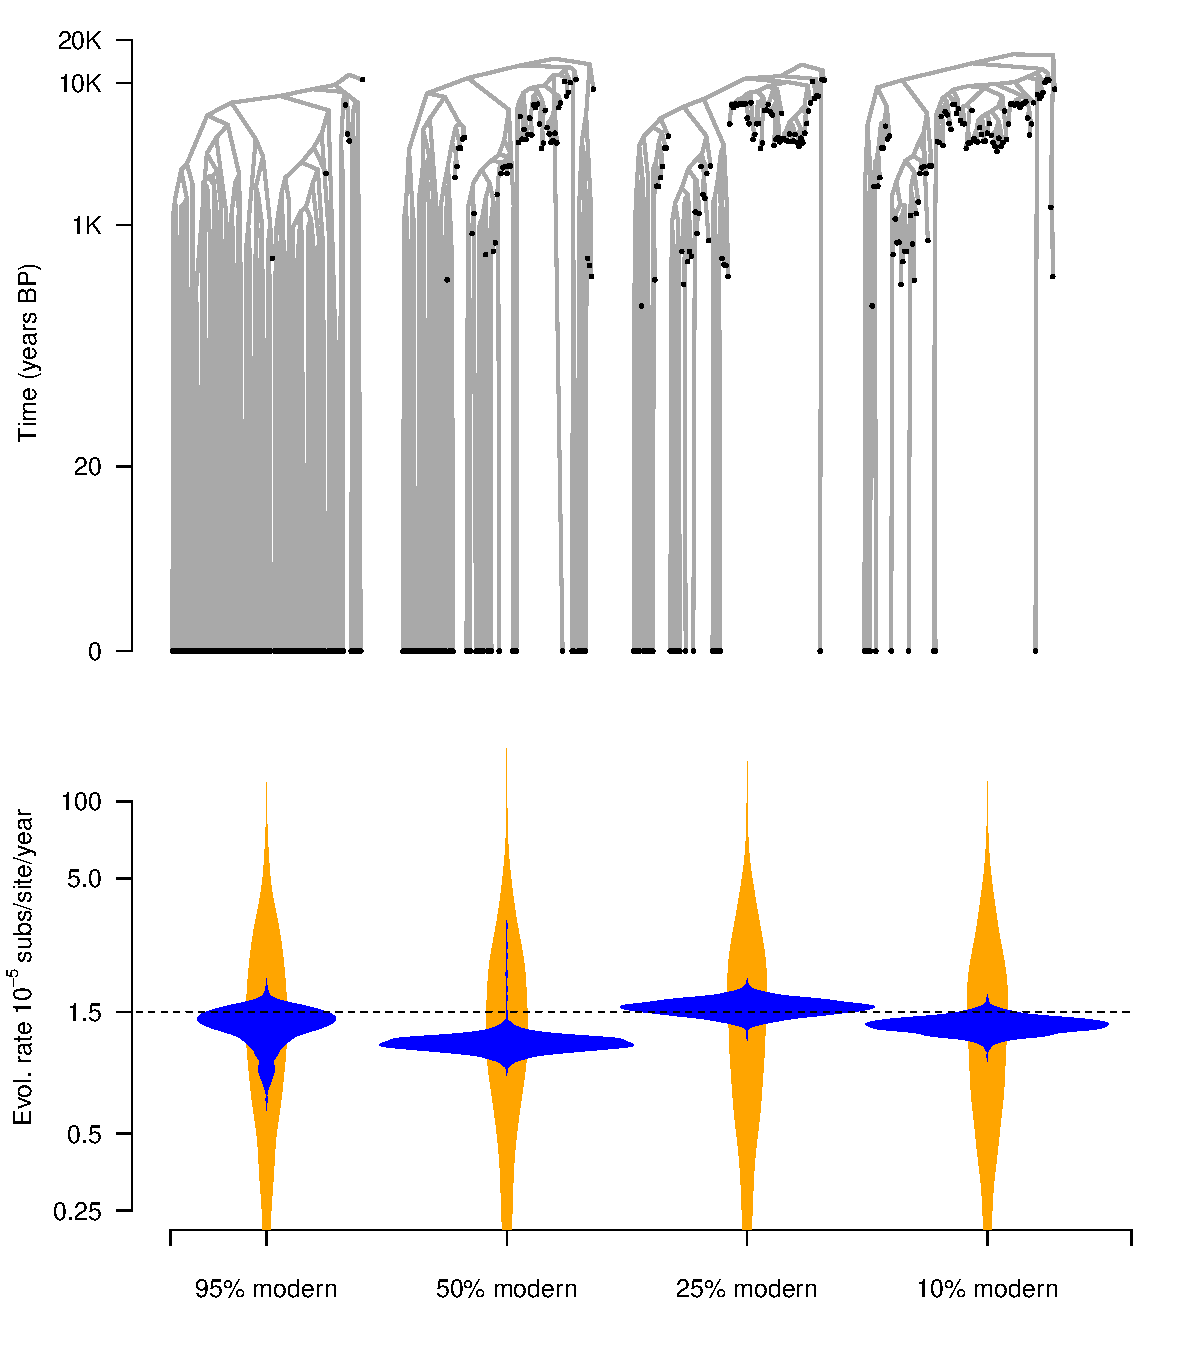
\includegraphics[scale=0.7, angle=0]{empirical_results_biased.pdf}
        \caption{Results from empirical analyses of Hepatitis B virus (HBV) ancient DNA data. The phylogenetic trees correspond to highest clade credibility trees from three analyses where the data were subsampled to include an increasing number of ancient samples. First, we consider a data set for which the samples are 95\% modern and the remaining 5\% being the most ancient. Then, we reduce the number of modern samples to 50\%, 25\% and 10\%, and the rest being ancient. Note that the sampling window is constant because we always retain the most ancient samples. In all cases the data sets consist of 100 genome samples. The violin plots show the posterior distribution of the evolutionary rate in blue and its corresponding prior in orange. The dashed line shows the mean evolutionary rate estimate from the complete data set.}
        \label{figure:Fig7}
    \end{center}
    %		\centering
\end{figure}

\section{Materials and methods}
\subsection{Simulations}
\subsubsection{Data generation}
We simulated phylogenetic trees and the evolution of nucleotide sequences to assess the impact of varying the sampling window and temporal sampling bias. We parameterised our simulations to resemble an HBV population evolving over 10,000 years before present, as described by \cite{kocher2021ten}. 

We generated phylogenetic trees under a coalescent process in which the population size has been constant over time using the package ReMaster \citep{vaughan2024remaster}, part of the BEAST 2 (version 2.7) software. We set the population size to 5,000, which results in trees with an average age of about 10,000 time units (years). The number of samples (i.e. tips) drawn from the trees and their ages was defined in ReMaster, according to the simulation scenario described below.

The simulation of sequence data requires trees with branch lengths in units of subs/site, instead of time. For this purpose, we multiplied the branch lengths of the simulated time tree with the rate of evolution, a lognormally distributed random variable with parameters $\mu=log(1.5\times10^{-5}) - \frac{0.25^2}{2}$ and $\sigma=0.25$. This procedure equates to simulating an uncorrelated relaxed molecular clock model with an underlying lognormal distribution \citep{drummond2006relaxed} with mean of $1.5\times10^{-5}$ subs/site/year and a standard deviation of 0.25 subs/site/year. Because we multiply the branch lengths in units of years by a variable in subs/site/year, the resulting trees have branch lengths in units of subs/site, formally known as phylograms, in contrast to chronograms where the branch lengths correspond to time.   We obtained sequence alignments using the R package phangorn (v2.8.1) \citep{schliep2011phangorn}, according to a HKY+$\Gamma_4$ substitution model, with parameters $\kappa=2$, $\alpha=4$, and equal base frequencies. The alignments consisted of 3,200 nucleotides to match the average genome size of HBV.

We considered the expected phylodynamic threshold of our data to be about 20 years. For our simulations where we varied the sampling window, we set the ages of 100 tips to be sampled at present (all have an age of 0), or to be drawn from a uniform distribution between 0 and 10 (1/2 of the expected phylodynamic threshold), 0 and 20, 0 and 200, or 0 and 2,000. 

To investigate the impact of temporal sampling bias we initially simulated trees with 500 tips with sampling times distributed in 5 time points, with 100 tips per time point. The distribution of sampling times followed an exponential distribution with mean of 4,000, such that sampling times were concentrated towards the present. We simulated these complete trees in ReMaster. We followed the procedure above to simulate a molecular clock model and sequence alignments. 

We conducted two sampling schemes for the trees with 500 tips: the `time-uniform' scheme consisted of drawing 20 samples from each time point, whereas the `time-biased' scheme included of mostly modern samples (90 from the present, and 5, 3, 1, and 1 from the remaining time points). For each simulation scenario we generated 100 replicates.

\subsubsection{Analysis of simulated data}
We analysed all data sets in BEAST 2 under a model that matched that used to generate the data: the HKY+$\Gamma_4$ substitution model, a uncorrelated relaxed molecular clock model with an underlying lognormal distribution, and a constant size coalescent tree prior. We used the default prior configuration in the program, except for the mean evolutionary rate and the population size of the coalescent ($\theta$) for which we specifically set a prior that was reasonable but not overly informative (table \ref{table:prior_distros}). For the simulations with varying sampling window width we investigated prior sensitivity in detail and thus we also analysed the data under a `misleading' prior configuration, where the prior density was deliberately concentrated on values that substantially differed from those used to generate the data.

\begin{table*}[h]
	\caption{Prior configuration for the molecular clock model and tree prior. The substitution model parameters had the default priors in BEAST 2. Note that the mean of the $\Gamma$ distribution here is $shape/rate$ and that the expected age of the root of a tree under a constant size coalescent is $2\times \theta$.} 
	\begin{center} 
		\label{table:prior_distros}
		\begin{tabular}{ c|c|c }
			Parameter & `Reasonable' prior & `Misleading' prior \\
			\hline
			 Coalescent population size ($\theta$) & $Exponential(mean=5,000)$ & $Exponential(mean= 50,000)$\\
			Molecular clock mean rate (M) & $\Gamma(shape=1.5, rate=10^5)$ & $\Gamma(shape=1.5, rate=10^6)$ \\
		\end{tabular}
	\end{center}	%\vspace{-0.4cm}
\end{table*}

Using the values from table \ref{table:prior_distros}, under the reasonable prior the mean of the lognormal distribution of branch rates has an average of $1\times 10^{-5}$ subs/site/year, with a 95\% quantile width of $1.1\times 10^{-6}$ to $4.7\times10^{-5}$, and the expected height of the root node is roughly 10,000 years (expected time to coalescent=$2\times \theta$ for an ultrametric tree, see \cite{nordborg2019coalescent}). In contrast, under the misleading prior the average evolutionary rate (mean of the lognormal distribution) is much lower, at $1\times10^{-6}$ subs/site/year, a 95\% quantile width of $1.1\times10^{-7}$ to $4.7\times10^{-6}$, and with an expected height of the root node of 100,000 years. In all cases we set the sampling times for calibration. In the case of ultrametric trees, sampling times are set to the present, such that all calibration information is provided by the prior.

We used Markov chain Monte Carlo (MCMC) to sample the posterior distribution. We set the chain length to $10^{8}$ steps, sampling every $5\times10^{4}$ steps. We deemed sufficient sampling by verifying that the effective sample size was at least 200, by using the R package CODA (version 0.19) \citep{plummer2006coda}. When this criterion was not met we extended the chain length to $5\times10^{8}$ steps. 

Our simulations with varying sampling window width used two possible prior configurations. To assess their impact we drew MCMC samples from the marginal prior of the evolutionary rate and the height of the root node. That is, the prior for a given parameter integrating over the prior in other parameters, the number of tips, and their heights. We obtained such samples by setting the option \texttt{sampleFromPrior="true"} in the input xml files in BEAST 2, which conducts the MCMC while ignoring the phylogenetic likelihood.

\subsubsection{HBV empirical data}
We selected a complete genome data set of HBV published by \cite{kocher2021ten}. The complete alignment included 232 genomes of length 3,344 nucleotides, with 1,807 variable sites, and 1,498 site patterns. The sampling times ranged from the present to 10,535 years before present. To investigate the impact of varying the sampling window and on temporal sampling bias we subsampled the data as described in our Results section. We analysed each data set using the same model and prior settings as in our simulations, including the use of the reasonable and misleading prior configuration.

\section{Data availability}
Computer code, analysis files, and data sets in this study are available at:

\url{https://github.com/sebastianduchene/phylo_threshold_code_data}

\section{Competing interests}
None.


\section{Acknowledgments}
Pending.



%\bibliographystyle{plain}
\bibliography{References}

\end{document}